\que{Одномерная оптимизация с использованием производной: методы средней точки,
хорд и касательных.}
Пусть дана система, вообще говоря, нелинейных уравнений $ \mathbf{F}(\mathbf{x}) =
\mathbf{0}$. Задача состоит в отыскании её приближённых решений.

\subsubsection{Метод касательных (Ньютона)}
\begin{alg}[одномерная версия] Требуется решить нелинейное уравнение $ f(x) = 0
  $ с погрешностью $ \varepsilon $.
  \begin{enumerate}
    \item Берётся произвольную точку $ x_0 $ области определения $ f $.
    \item Решается вспомогательная линейная задача
      \begin{equation}\label{eq:newton1}
        f(x_n) + f'(x_n)(x-x_n) = 0.
      \end{equation}
      \begin{enumerate}
        \item Если решение существует, то решение задачи берётся принимается за следующее приближение, 
          \[
            x_{n+1} = x_n - f(x_n)/f'(x_n).
          \]
        \item В ином случае алгоритм следует начать заново с другой точкой.
      \end{enumerate}
    \item Вычисления могут быть прерваны, когда 
      \begin{equation}\label{eq:newton-pogr}
      |x_n - x_{n-1}| < \varepsilon.
    \end{equation}
  \end{enumerate}
\end{alg}

\paragraph{Обоснование.} Метод имеет наглядную геометрическую интерпретацию. В
уравнении \eqref{eq:newton1}
ищется пересечение касательной в точке $ x_n $ с осью $ Ox $. 
\begin{figure}[h]
  \centering
  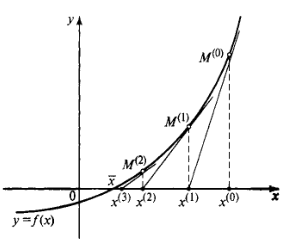
\includegraphics[width=0.4\textwidth]{img/newton.png}
  \label{fig:newton}
\end{figure}
Таким образом, каждая итерация всё более приближает $ x_n $ к $ \bar x $
(обозначение истинного корня).

Само уравнение \eqref{eq:newton1} есть так называемая \emph{линеаризация}
данного уравнения $ f(x) $ --- мы заменяем исходное уравнение первым
приближением и корень этого приближения.

\begin{theorem}
  Пусть $ \bar x $ --- простой корень уравнения $ f(x) = 0$, в некоторой
  окрестности которого функция дважды дифференцируема. Тогда найдётся такая $
  \sigma $-окрестность $ \bar x $, что метод Ньютона с начальной точкой из этой
  окрестности не выходит за её пределы и справедлива оценка 
  \begin{equation}\label{eq:newton2}
    |x_{n+1} - \bar x| \leqslant \sigma^{-1}|x_n - \bar x|^2,
  \end{equation}
  означающая, что метод сходится с \emph{квадратичной скоростью}.
  Прямым следствием является априорная оценка  
  \begin{equation}\label{eq:newton3}
    |x_n - \bar x| \leqslant \sigma q^{2n},
  \end{equation}
  в которой $ q =\sigma^{-1}|x_0 - \bar x| $.
\end{theorem}
\begin{proof}
  По определению простого корня $ f'(\bar x) \neq 0 $. Используем непрерывность
  производных и возьмём такую $ \delta_0 $-окрестность, где $ 0 < \alpha
  \leqslant |f'(x)| $, $ |f''(x)| \leqslant \beta $ и положим $ \sigma =
  \min\{\delta_0, 2\alpha/\beta\} $. 

  Пусть теперь $ x_n \in (\bar x - \sigma, \bar x + \sigma) $. По формуле
  Тейлора с остаточным членом имеем  
  \[
      0 = f(x_n) + f'(x_n)(\bar x - x_n) + \frac{f'(\xi)}{2}(\bar x - x_n)^2,
  \]
 в котором $ \xi \in (\bar x - \sigma, \bar x + \sigma) $. Вычтем отсюда
 равенство $ 0 = f(x_n) + f'(x_n)(x_{n+1} - x_n) $ и получим неравенство 
 \[
   \alpha|x_{n+1} - \bar x| \leqslant  \frac{\beta}{2}|x_n - \bar x|^2.
 \]
\end{proof}

\begin{theorem}
  Пусть выполнены условия прошлой теоремы и $ |x_0 - \bar x| < \sigma/2 $. Тогда
  для всех $ n \leqslant 1 $ верна оценка  
  \[
    |x_n - \bar x| \leqslant |x_n - x_{n-1}|.
  \] 
\end{theorem}
\begin{proof}
  Из \eqref{eq:newton3} следует, что  
  \[
    |x_{n-1} - \bar x| \leqslant \sigma q^{2^{n-1}} \leqslant \sigma q = |x_0 -
    \bar x| < \sigma/2.
  \]
  Применяя теперь оценку \eqref{eq:newton2}, получим  
  \[
    2|x_n - \bar x| \leqslant 2\sigma^{-1}|x_{n-1} - \bar x|^2 \leqslant
    |x_{n-1} - \bar x| \leqslant |x_{n-1} - x_n| + |x_n - \bar x|.
  \]
\end{proof}
Из этой теоремы непосредственно следует условие остановки
\eqref{eq:newton-pogr}.


\subsubsection{Метод хорд (секущих)}
Замена в формуле метода Ньютона производной $ f'(x_n) $ приближением в виде
секущей приводит к
расчётной формуле
\[
  x_{n+1} = x_n - \frac{x_{n-1} - x_n}{f(x_{n-1}) - f(x_n)} f(x_n).
\]
\begin{figure}[h]
  \centering
  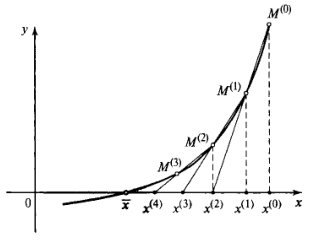
\includegraphics[width=0.4\textwidth]{img/chord.png}
  \label{fig:chord}
\end{figure}
Заметим, что метод двушаговый. В том числе требуется два начальных значения.
\begin{theorem}
  Пусть $ \bar x $ --- простой корень уравнения $ f(x) = 0 $, в некоторой
  окрестности которого функция $ f $ дважды непрерывно дифференцируема, причём
  $ f''(\bar x) \neq 0 $. Тогда существует $ \sigma $-окрестность корня $ \bar x
  $ такая, что при произвольном выборе приближений $ x_0 $ и $ x_1 $ из этой $
  \sigma $-окрестности метод секущих сходится с оценкой  
  \[
    |x_{n+1} - \bar x| \leqslant c |x_n - \bar x|^p, 
    \quad p = \frac{\sqrt 5 + 1}{2}.
  \]
\end{theorem}

Заметим, что метод Ньютона требует двух вычислений --- значения $ f $ и значения
$ f' $ --- на каждом шаге, а метод секущих одно. Кроме того, метод секущих
сходится быстрее. Однако он обладает, вообще говоря, только локальной
сходимостью.


\subsubsection{Метод средней точки}
Задача состоит в поиске стационарных точек (потенциально точек экстремума).
Алгоритм аналогичен стандартному поиску корней, но для производной.
\begin{alg}
  Дан отрезок $ [a_0,b_0] $, на котором требуется найти стационарную точку с
  заданной погрешностью $ \varepsilon $. (Предполагается, что $ f'(a_0) < 0 <
  f'(b_0) $, а также непрерывность функции и её производной).
  \begin{enumerate}
    \item Берётся середина $ c_k := \frac{a_k + b_k}{2} $ отрезка $ [a_k, b_k] $.
    \item Рассматривается три случая:
      \begin{enumerate}
        \item $ f'(c_k) = 0 $. Тогда алгоритм окончен.
        \item $f'(c_k) < 0$. Тогда полагаем $ a_k = c_{k-1} $, $ b_k = b_{k-1}
          $.
        \item $f'(c_k) > 0$. Тогда полагаем $ a_k = a_{k-1} $, $ b_k = c_{k-1}
          $.
      \end{enumerate}
    \item Переходим к шагу 1.
    \item Остановиться следует, когда $ b_k - a_k = \frac{b - a}{2^k} < \varepsilon $.
  \end{enumerate}
\end{alg}
